%%%%%%%%%%%%%%%%%%%%%%%%%%%%%%%%%%%%%%%%%%%%%%%%%%%%%%%%%%%%%%%%%%
%%%%%%%% ICML 2015 EXAMPLE LATEX SUBMISSION FILE %%%%%%%%%%%%%%%%%
%%%%%%%%%%%%%%%%%%%%%%%%%%%%%%%%%%%%%%%%%%%%%%%%%%%%%%%%%%%%%%%%%%

% Use the following line _only_ if you're still using LaTeX 2.09.
%\documentstyle[icml2015,epsf,natbib]{article}
% If you rely on Latex2e packages, like most moden people use this:
\documentclass{article}

% use Times
\usepackage{times}
% For figures
\usepackage{graphicx} % more modern
%\usepackage{epsfig} % less modern
\usepackage{subfigure} 

% For citations
\usepackage{natbib}

% For algorithms
\usepackage{algorithm}
\usepackage{algorithmic}
\usepackage{amsmath}
\usepackage{todonotes}

% As of 2011, we use the hyperref package to produce hyperlinks in the
% resulting PDF.  If this breaks your system, please commend out the
% following usepackage line and replace \usepackage{icml2015} with
% \usepackage[nohyperref]{icml2015} above.
\usepackage{hyperref}

% Packages hyperref and algorithmic misbehave sometimes.  We can fix
% this with the following command.
\newcommand{\theHalgorithm}{\arabic{algorithm}}

% Employ the following version of the ``usepackage'' statement for
% submitting the draft version of the paper for review.  This will set
% the note in the first column to ``Under review.  Do not distribute.''
% \usepackage{icml2015} 

% Employ this version of the ``usepackage'' statement after the paper has
% been accepted, when creating the final version.  This will set the
% note in the first column to ``Proceedings of the...''
\usepackage[accepted]{icml2015}


% The \icmltitle you define below is probably too long as a header.
% Therefore, a short form for the running title is supplied here:

% Saving space by deleting running title (does this actually save space?)
%\icmltitlerunning{Submission and Formatting Instructions for ICML 2015}

\begin{document} 

\twocolumn[

% Saving space by deleting title
%\icmltitle{Submission and Formatting Instructions for \\ 
%           International Conference on Machine Learning (ICML 2015)}

% It is OKAY to include author information, even for blind
% submissions: the style file will automatically remove it for you
% unless you've provided the [accepted] option to the icml2015
% package.
\icmlauthor{Lucas Manuelli}{manuelli@mit.edu}
\icmladdress{Massachusetts Institute of Technology}
\icmlauthor{Pete Florence}{peteflo@mit.edu}
\icmladdress{Massachusetts Institute of Technology}

% You may provide any keywords that you 
% find helpful for describing your paper; these are used to populate 
% the "keywords" metadata in the PDF but will not be shown in the document
\icmlkeywords{6.867, machine learning}

\vskip 0.3in
]

% Saving space by deleting abstract
%\begin{abstract} 
%The purpose of this document is to provide both the basic paper template and
%submission guidelines.
%\end{abstract} 

\section{Introduction}
In this project we evaluate the ability of several reinforcement learning methods to autonomously drive a car through a cluttered environment. We don't assume a map of the environment a priori but rather rely on our sensor (in this case a LIDAR) to make control decisions. A standard approach to solving this problem would require building up a map of the environment, possibly using an occupancy grid, and then planning a collision free path through this estimated map using a planner such as RRT*. On the other hand one notes that simple output feedback controllers such as Braitenburg controllers, can be quite effective for obstacle avoidance tasks. Guided by this example we want to see how reinforcement learning performs in learning an output feedback controller.

\section{Experiment Setup and Simulation Environment}

\subsection{Car Model}

For our car model we consider a simplified Dubin's car model. The location of the vehicle is described by $(x,y,\theta)$, where $(x,y)$ denote cartesian position and $\theta$ denotes the orientation. For our purposes we suppose that we can control the derivative of the orientation, namely our control is $u = \dot{\theta}$. We also suppose a fixed speed $v$. Then the dynamics of the vehicle are given by

%
%
\begin{align}
\dot{x} &= v \cos(\theta) \\ 
\dot{y} &= v \sin(\theta)\\ 
\dot{\theta} &= u
\end{align}
%
%
%
\subsection{Sensor Model}
For our sensor model we use a LIDAR. Namely it consists of $N$ beams spread evenly over the field of view $[\theta_min,\theta_max]$. Each laser has a maximum range of $d_{max}$. The $n^th$ laser then returns $x_n$, which the distance to the first obstacle it encounters, or $d_{max}$ if no obstacle is detected. Then one laser measurement can be summarized as $X = (x_1,\ldots,x_N)$.


\subsection{Simulation Environment}

Our software stack is integrated with a robotics visualization tool called Director \todo{director citation}. We use the director code for visualization and raycasting. This is the only external code that we use. Our simulation environment is written in python. We have a main class called simulator which combines together several other modules, e.g. car, sensor, world, controller, reward, sarsa etc, to construct a working simulation class. All of this code was written by us for the project. As mentioned before, the only fundamental pieces of code that we didn't write were the visualization tools and the raycasting method which we use for computing our sensor model. One nice feature of the Director application is that it uses Visualization Toolkit as the underlying graphics engine, and thus our raycast calls are actually in C++ and thus very efficient. We use a timestep of $dt = 0.05$ in all our experiments.

\subsection{Default Controller}
\label{default_controller}
Describe it here, maybe this is where we should introduce the $\phi(\cdot)$ function.

\section{Dynamic Programming: SARSA and Q-Learning}
Two of the most popular methods in reinforcement learning are SARSA and Q-Learning. These methods both aim to find the optimal policy of a dynamic programming problem. Thus the first step is to reformulate our problem as a dynamic programming problem. 

\subsection{Dynamic Programming Formulation}
The first step to formulating our as a dynamic programming problem is to define a ``state.'' Let $S_c = (x,y,\theta)$ be the state of the car, and let $X  = (x_1,\ldots,x_n)$ be the sensor state. Then let $S = (S_c,X)$ be our ``state''. Since this is not a state in the true sense of the word let us call it a reward state. Next we need to define our action set. In principle our model has continuous action set. However, for the purposes of SARSA and Q-Learning it much easier to have a discrete action space. Thus we restrict ourselves to $a \in \{-4,0,4\} = \mathcal{A}$, which correspond to left, straight, and right actions. Let $\theta_n$ be the angle of $n^th$ laser where $\theta_n = 0$ corresponds to straight ahead. Now we need to define the reward function. First define weights
%
%
\begin{equation}
w_n = r_0 + r_1 \cos(\theta_n)
\end{equation}
%
%
Also define
%
%
\begin{equation}
\phi(x_n) = \begin{cases}
\min(1/x_n, C_{max}) & x_n < d_{max}\\
0 & x_n = d_{max} 
\end{cases}
\end{equation}
%
%
Then $\phi$ has the effect of amplifying short distance measurements. Let $W = (w_1,\ldots,w_N), \phi(X) = (\phi(x_1),\ldots,\phi(x_n))$ Then define the reward $R(S,a)$ as
%
%
\begin{equation}
R(S,a) = C_{action} |a| + \langle W, \phi(X) \rangle
\end{equation}
%
%
where $C_{action}$ is an action cost. Finally if the car is currently in collision with an obstacle, i.e. some laser $x_n$ is reading less than $d_{min}$ then we set $R(S,a) = C_{collision}$.

Now let us think about why this may be a reasonable reward function for our objective, which is obstacle avoidance. One should think of $r_0,r_1, C_{action}, C_{collision} < 0$ and $C_{max} > 0$. Then we see that the components of $\phi(X)$ increase as we get close to obstacles. And they increase as the inverse of the distance to the obstacle. Thus this is penalizing getting too close to obstacles. Now consider the weights $W$. They have the following form \todo{include picture}. This means that it's worse to have obstacles in front of you than off to the side. The action cost is to encourage the car to drive straight rather than spin around in circles. Finally since we are interested in obstacle avoidance we impose a large penalty if the car does crash into an obstacle.

The reason we have $\phi(X)$ and the weights $W$ is reward shaping. In reality all we care about is not crashing into obstacles, but it helps the algorithms to converge if the rewards ``guide'' them towards staying away from obstacles, e.g. if the reward is higher the further you are from the obstacles. 

Now that we have the reward function we can formulate our problem as a dynamic program. The problem is to find the policy $\pi:S \to \mathcal{A}$ to solve
%
%
\begin{equation}
\max_{\pi} E_{\pi} \left[ \sum_{t \geq 0} \gamma^t R(S_{t+1}, a_t) \right]
\end{equation}
%
%
The expectation is over the reward states that result from taking actions according to policy $\pi$. Here $\gamma \in (0,1)$ is a discount factor. In a standard dynamic programing framework the state $S_t$ would be markov. That is, future states depend only on the current state and future actions. In our case however our reward state is non-markov since the map of the world is not included as part of our state. 

\subsection{SARSA}
The difficulty with applying standard dynamic programming techniques to the current problem is that it is hard to write down the transition law $(S_t,a_t) \to S_{t+1}$ since this requires knowing how the sensor measurements will evolve. The SARSA technique allows us to circumvent this problem if we have access to runs/simulations of the true system. The Q-Values are defined as 
%
%
\begin{equation}
q_{\pi}(S,a) = E_{\pi} \left[ \sum_{k \geq 0} \gamma^k R(S_{t+k+1}, a_{t+k}) | S_t = s, A_t = a \right]
\end{equation}
%
%
Then if we knew the Q-values we could choose the best policy as 
%
\begin{equation}
\label{q-policy}
a = \arg \max_{a'} q_{\pi}(s,a) 
\end{equation}
%
The ultimate goal of SARSA($\lambda$). Is to find the optimal policy $\pi^*$. The approach is to estimate $q_{\pi^*}$. Then the optimal policy is found by appling equation (\ref{q-policy}). Using the Bellman equation for the Q-Values the SARSA($\lambda$) update is given by \todo{use algorithmic package to do description of SARSA() here }


In order to apply SARSA in the form described above we need to discretize the state-action space. In section \ref{sarsa_function_approximation} we describe an approach that doesn't require discretizing the state. In order for the SARSA algorithm to be effective without drastically increasing the training time, we must keep the size of the discretization relatively small. With this in mind we chose a discretization based on bins. The discretization is paramaterized by three parameters. $N_{inner}$, the number of inner bins, $N_{outer}$ the number of outer bins and $\beta_{cutoff}$, the cutoff distance between inner and outer bins. \todo{could use a picture here that describes the discretization}.


Bins are labeled with a $1$ if they are occupied. We have already discretized the action space into $\mathcal{A} = \{-4,0,4\}$. Thus the discretization of the state-action space lies in the space $\{0,1\}^{N_{inner} + N_{outer}} \times \mathcal{A}$. Thus it has size $2^{N_{inner} + N_{outer}} \times |\mathcal{A}|$.



\subsubsection{Results}

There are many parameters that must be chosen in order to run the SARSA lambda algorithm. We discuss some of the most important here and give intuition on how we chose them. Then we will analyse how varying a few key parameters (such as $\lambda$) around our baseline setup affects performance. show plots illustrating  Then we show plots of performance as we vary certain key parameters.

Two of the most important parameters are the number of bins $N_{inner}, N_{outer}$ in the discretization. You need enough bins that so that the state is informative enough to pass through relatively narrow gaps between obstacles. However adding more bins comes at the cost of increasing the size of the state space which can increase training time. In addition if a particular action-state pair is not visited sufficiently many times then that Q-value $Q(s,a)$ will not be a good approximation to the true Q-value, and hence control decisions taken based on that Q-value will not be optimal (and in fact will be quite poor usually). Through many experiments we found that $N_{inner} = 5, N_{outer} = 4$ provided good performance while keeping the size of the discretized state-action space relatively small at $2^9 * 3 = 1536$. Another set of parameters that had a large impact on performance were those of the cost function. It turned out to be important to balance the reward for staying away from obstacles with the penalty for using large control action, $C_{action}$. If $C_{action}$ was too small the controller could end up learning to spin in circles, see Section \ref{failure_modes} for more discussion of this problem. Alternatively if $C_{action}$ was too high the behavior would bias too much towards driving straight and wouldn't do enough to avoid obstacles. Another important parameter was the step size $\alpha$ in the SARSA update. It needs to be small enough so that the Q-Value estimates don't diverge. However, if it is too small then the Q-values are updated only a small amount in each iteration and convergence would take a long time. For the discrete state-action case we found that $\alpha = 0.2$ worked well, although it is difficult to evaluate what the ``correct'' step size is. See Table \todo{make a table with default parameter values, put it in the appendix} for our preferred set of parameters.

First we provide a qualitative discussion of the results of the Q-Learning using parameters from Table \todo{make a table with default parameter values, put it in the appendix}. We initialize all of the Q-value to zero and run the SARSA algorithm for 8000 seconds. Since our simulation timestep is $dt = 0.05$ this amounts to $8000/dt = 160,000$ iterations of the SARSA update. Our simulation runs at approximately $700$ Hz. Since it takes $20$ ticks of the simulator to complete one second this amounts to a simulation of 35 $\times$ normal speed. Thus this training takes approximately $3.8$ minutes. The controller that we get out of this performs reasonably well. Specifically it manages to drive around the obstacle field shown in figure \todo{picture of the obstacle field} at a reasonably high speed with mean time between crashes of \todo{figure this out, currently it is 600} 30 seconds. One thing to note is that this is much worse than the performance of our default controller described in section \ref{default_controller}. At the given car speed in this run the default controller can essentially drive around indefinitely without crashing. However, it's behavior is to make a hard turn as soon as it detects an obstacle. Thus it has a tendency to get trapped within an area just going in circles as in figure \todo{show figure}. Since the default controller turns very agressively it never will go through a small gap. On the other hand since our reward function penalizes taking control actions (by $C_{action}$) it rewards our controller for going straight. Thus the learned controller will continue to go straight in some situations where we are detecting obstacles, but they are not in our direct path see figure \todo{include graphic}. This is an interesting behavior that is learned. Thus qualitatively our learned controller turns much less than the default controller and thus doesn't tend to get stuck circling in one spot. Another interesting feature of the controller is that learns how to drive through narrow gaps, see figure \todo{include graphic}.

For a more quantitative analysis we can consider plots showing the average and discounted reward. The plots show that as time progresses the algorithm improves it's performance as is to be expected. Both the discounted reward and the run duration increase over time as the learning improves. 



Things to do
\begin{itemize}
\item Same parameters many runs, show the variance in the learning
\item Different lambdas, see if there is noticeable difference in performance.
\item Compare multiple runs for Q-Learning and SARSA, is one more consistent than the other?
\end{itemize}


\subsection{Watkins Q-Learning}

Q-Learning is almost the same as SARSA but with a slight variation in the update. While SARSA is an on-policy learning method (that is we are learning the Q-value for the current policy), Q-Learning is an off-policy method (we are learning the Q-Values under the optimal policy (even though we not currently controlling according that policy). The same preferred parameter set for SARSA given in Table \todo{reference} works well for Q-Learning also. The resulting controller exhibits similar qualitative performance to the SARSA controller described above. However the quantitative performance is a bit better.




\subsection{SARSA with function approximation}
\label{sarsa_function_approximation}
%
%
% \begin{align}
% &\delta \leftarrow R + \gamma Q(S',A') - Q(S,A)\\
% & Z(S,A) \leftarrow Z(S,A) + 1\\
% \text{for all } s \in \mathcal{S}, a \in \mathcal A
% \end{align}
% %
% %



\subsection{Failure Modes}
\label{failure_modes}
We end up spinning around in circles. Maybe this is because we are assuming we are Markov when really we are not?


 so that we penalize being close to obstacles, i.e. 

\section{Conclusion}

\section{Division of Labor}

\section{Figures}

\begin{figure}
\centering
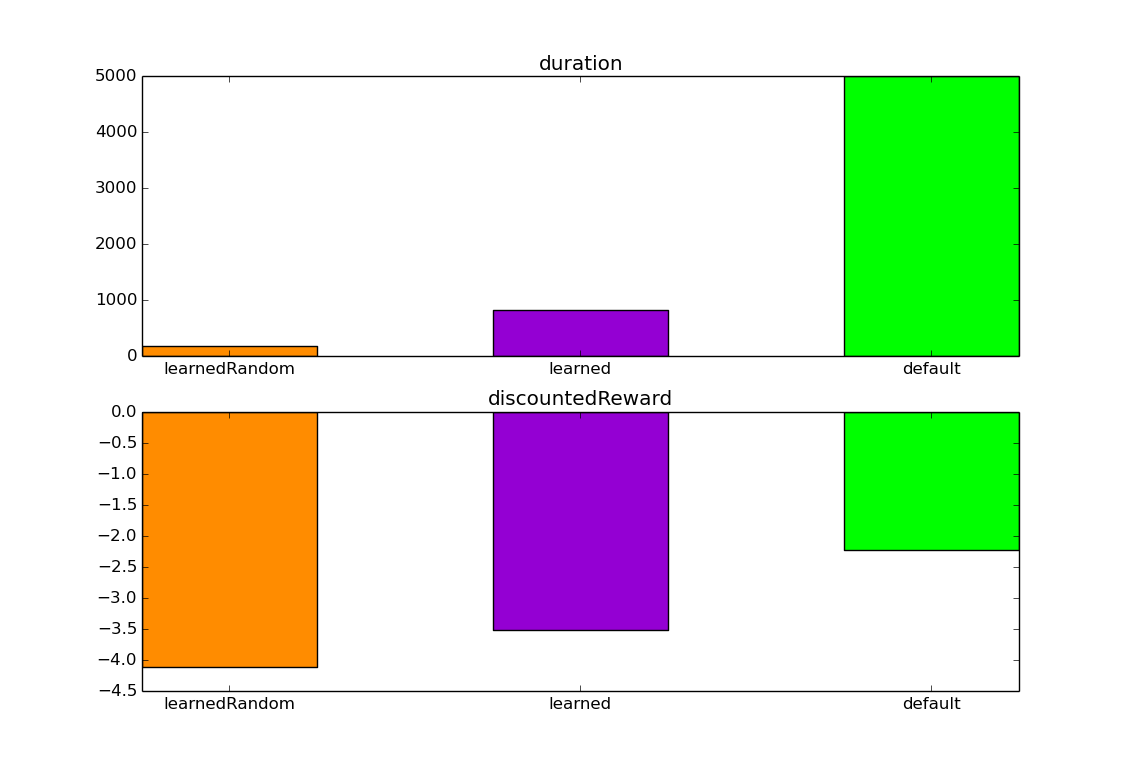
\includegraphics[scale=0.5]{figures/sarsaDiscrete_lam_0_7_6500_bar_all_controllers.png}
\caption{$\lambda = 0.7$}
\label{figures/sarsaDiscrete_lam_0_7_6500_bar_all_controllers.png}
\end{figure}

\begin{figure}
\centering
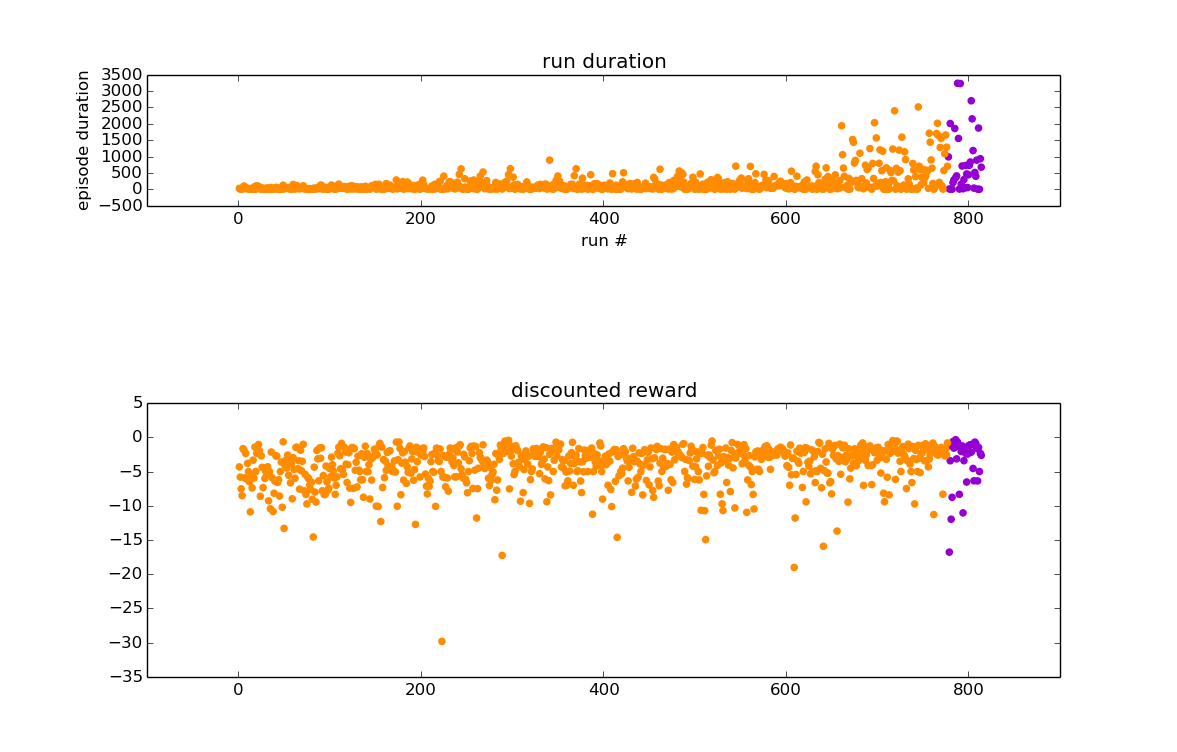
\includegraphics[scale=0.5]{figures/sarsaDiscrete_lam_0_7_6500_time_series_learned_controllers.png}
\caption{$\lambda = 0.7$}
\label{figures/sarsaDiscrete_lam_0_7_6500_time_series_learned_controllers.png}
\end{figure}



\bibliography{example_paper}
\bibliographystyle{icml2015}

\end{document} 


% This document was modified from the file originally made available by
% Pat Langley and Andrea Danyluk for ICML-2K. This version was
% created by Lise Getoor and Tobias Scheffer, it was slightly modified  
% from the 2010 version by Thorsten Joachims & Johannes Fuernkranz, 
% slightly modified from the 2009 version by Kiri Wagstaff and 
% Sam Roweis's 2008 version, which is slightly modified from 
% Prasad Tadepalli's 2007 version which is a lightly 
% changed version of the previous year's version by Andrew Moore, 
% which was in turn edited from those of Kristian Kersting and 
% Codrina Lauth. Alex Smola contributed to the algorithmic style files.  
